\chapter{Pattern Mining}
\label{ch:capitolo2}
% To perform this task, continuous attributes were discretized based on their distributions, 
% aiming for bins that were both semantically meaningful and reasonably balanced in size. 
% The selected numerical attributes (not normalized) for the pattern mining task, along with their binning, are the following: \\ \\ 
% \begin{table}[H]
% \centering
% \begin{tabular}{ll}
% \toprule
% \textbf{Attribute} & \textbf{Binning} \\
% \midrule
% \texttt{runtimeMinutes} & VeryLowRTM (1-30), LowRTM (31-60), MediumRTM (61-90), HighRTM (91-220) \\
% \texttt{rating} & VeryLowR (1-3), LowR (4-6), MediumR (7), HighR (8), VeryHighR (9-10) \\
% \texttt{totalCredits} & VeryLowC (0-15), LowC (16-35), MediumC (36-65), HighC (66-15742) \\
% \bottomrule
% \end{tabular}
% \caption{Binning of the continuous attributes}
% \end{table}
% Regarding discrete attributes, \texttt{titleType} was considered for this task, kept in its original form. 
% On the other hand, the values of each of the 7 attributes \texttt{countryOfOrigin\_[continent code]}\footnote{see subsection 1.1.3 for the list of the features} were binarized into:
% \begin{itemize}
%     \item \texttt{not\_from\_[continent code]}: when the value of the attribute is 0
%     \item \texttt{is\_from\_[continent code]}: when the value of the attribute is $\geq$ 1
% \end{itemize}
% Binarization was preferred over creation of multiple bins, as it allows for a more linear interpretation of the results. 
% An attempt was performed to include genres; however, this did not lead to more interesting results.

To perform this task, some attributes needed preprocessing. As for discrete features, the values of each of the 7 attributes \texttt{countryOfOrigin\_[continent code]}\footnote{see subsection 1.1.3 for the list of the features} were binarized into:
\begin{itemize}
    \item \texttt{not\_from\_[continent code]}: when the value of the attribute is 0
    \item \texttt{is\_from\_[continent code]}: when the value of the attribute is $\geq$ 1
\end{itemize}
Binarization was preferred over creation of multiple bins, as it allows for a more linear interpretation of the results. 
On the other hand, \texttt{titleType} was kept in its original form.  An attempt was performed to include genres; however, this did not lead to more interesting results.
\\

Regarding continuous attributes, they were discretized based on their distributions, 
aiming for bins that were both semantically meaningful and reasonably balanced in size. 
The selected numerical attributes (not normalized) for the pattern mining task, along with their binning, are the following:
\begin{table}[H]
\centering
\begin{tabular}{ll}
\toprule
\textbf{Attribute} & \textbf{Binning} \\
\midrule
\texttt{runtimeMinutes} & VeryLowRTM (1-30), LowRTM (31-60), MediumRTM (61-90), HighRTM (91-220) \\
\texttt{rating} & VeryLowR (1-3), LowR (4-6), MediumR (7), HighR (8), VeryHighR (9-10) \\
\texttt{totalCredits} & VeryLowC (0-15), LowC (16-35), MediumC (36-65), HighC (66-15742) \\
\bottomrule
\end{tabular}
\caption{Binning of the continuous attributes}
\end{table}

\section{Extraction and discussion of frequent patterns}\label{sec:freq_patterns}
\begin{figure}[H]
    \centering
    % First subfigure
    \begin{subfigure}{0.49\textwidth}
        \centering
        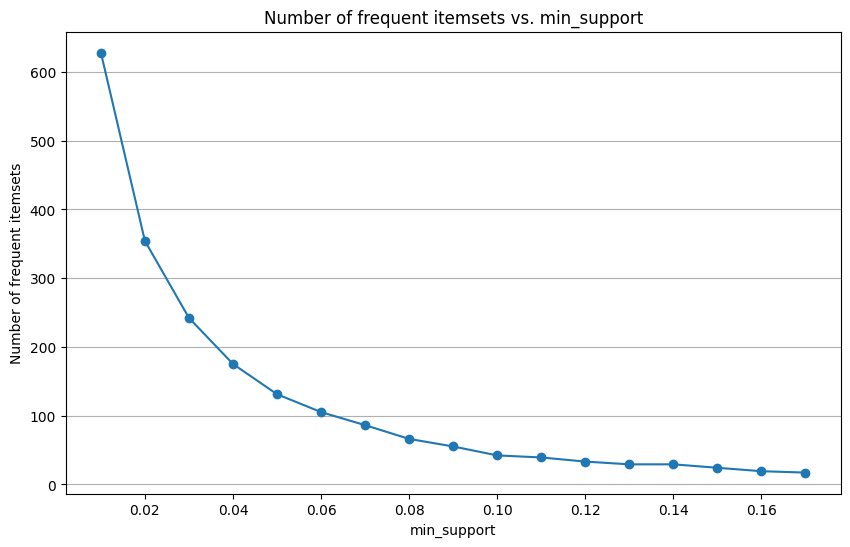
\includegraphics[width=0.98\textwidth]{plots/5_min_sup.png}     %se teniamo 0.65 ci sta sotto la tabella delle continuous
        \caption{Plot of frequent itemsets with varying \textit{support}}
        \captionsetup{width=0.9\linewidth, justification=centering}
        \label{fig:min_sup}
    \end{subfigure}
    \begin{subfigure}{0.49\textwidth}
        \centering
        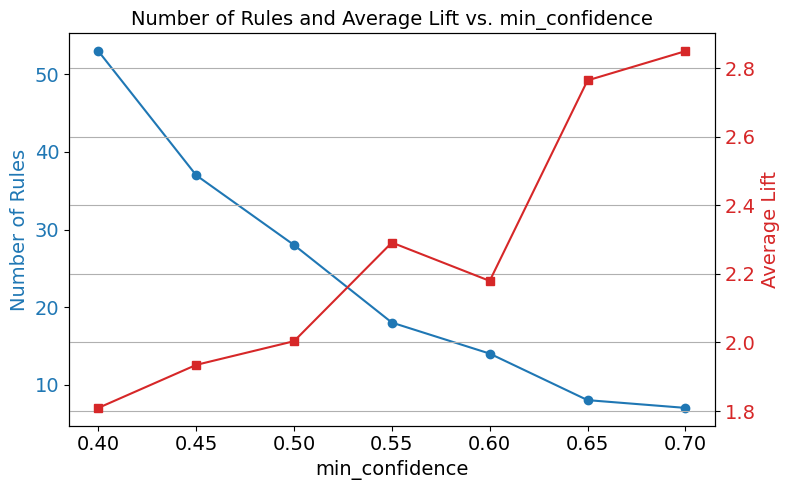
\includegraphics[width=0.98\textwidth]{plots/5_min_conf.png}     %se teniamo 0.65 ci sta sotto la tabella delle continuous
        \caption{Plot of lift and number of rules with varying \textit{confidence}}
        \captionsetup{width=0.9\linewidth, justification=centering}
        \label{fig:min_conf}
    \end{subfigure}
    \captionsetup{justification=centering}
    \caption{Plots of minimum support and confidence - \textit{Apriori} algorithm}
    \label{fig:distrib}
\end{figure}
\textit{Apriori} was the algorithm chosen to extract frequent patterns. 
Figure~\ref{fig:min_sup} shows how the number of frequent itemsets changes with support values ranging from 0.01 to 0.18. 
The curve of the plot begins to flatten between 0.08 and 0.1, so a support value of 0.08 was selected, resulting in 66 frequent patterns.\\
It is interesting to observe the top frequent itemsets of size 1, 2, and 3, as shown in Table~\ref{tab:top-itemsets}. 
From the itemset of size 1 it was noticed that approximately 48.5\% of the objects in the dataset are from North America, highlighting the prevalence of this region.

\begin{minipage}{0.42\textwidth}
The size-2 itemset reveals that 1/4 of the objects is both from North America and has a very low runtime.
This pattern becomes more specific in the top size-3 itemset, where almost 10\% of the data corresponds to TV episodes with both characteristics.
\end{minipage}
\hfill
\begin{minipage}{0.56\textwidth}
\centering
\begin{tabular}{ccl}
\toprule
\textbf{Size} & \textbf{Support} & \textbf{Itemsets} \\
\midrule
1 & 0.485 & (is\_from\_NA) \\
2 & 0.204 & (VeryLowRTM, is\_from\_NA) \\
3 & 0.094 & (tvEpisode, VeryLowRTM, is\_from\_NA) \\
\bottomrule
\end{tabular}
\captionof{table}{Top itemsets of sizes 1, 2, and 3}
\label{tab:top-itemsets}
\end{minipage}


% It is interesting to observe the top frequent itemsets of size 1, 2, and 3, as shown in Table 5.2. 
% From the itemset of size 1 it was noticed that approximately 48.5\% of the objects in the dataset are from North America, highlighting the prevalence of this region. 
% The size-2 itemset reveals that 1/4 of the objects is both from North America and has a very low runtime. 
% This pattern becomes more specific in the top size-3 itemset, where almost 10\% of the data corresponds to tv episodes with both characteristics.

% \begin{table}[h]
% \centering
% \begin{tabular}{ccl}
% \toprule
% \textbf{Size} & \textbf{Support} & \textbf{Itemsets} \\
% \midrule
% 1 & 0.485 & (is\_from\_NA) \\
% 2 & 0.204 & (VeryLowRTM, is\_from\_NA) \\
% 3 & 0.094 & (tvEpisode, VeryLowRtm, is\_from\_NA) \\
% \bottomrule
% \end{tabular}
% \caption{Top Itemsets of 1, 2, 3 sizes}
% \end{table}



\section{Extraction of rules}\label{sec:rules}
After extracting the frequent patterns, association rules were generated.
To find a value of \textit{confidence} that balances the number of rules and their strength (measured with \textit{lift}), 
the plot in Figure\ref{fig:min_conf} was analysed. A \texttt{min\_confidence} of 0.55 was selected, guaranteeing an average \textit{lift} of 2.3 and 
a significant number of rules, i.e. 18. The top 10 rules extracted (ranked by lift) are:
\begin{table}[h]
\centering
\begin{tabular}{cllcccccc}
\toprule
\textbf{Rule} & \textbf{Antecedents} & \textbf{Consequents} & \shortstack{\textbf{Ant.}\\\textbf{Sup.}} & \shortstack{\textbf{Cons.}\\\textbf{Sup.}} & \textbf{Sup.} & \textbf{Conf.} & \textbf{Lift} \\
\midrule
0 & (short) & (VeryLowC, VeryLowRTM) & 0.160 & 0.128 & 0.093 & 0.583 & 4.568 \\
1 & (VeryLowC, VeryLowRTM) & (short) & 0.128 & 0.160 & 0.093 & 0.731 & 4.568 \\
2 & (HighRTM) & (movie) & 0.177 & 0.319 & 0.154 & 0.866 & 2.719 \\
3 & (is\_from\_NA, short) & (VeryLowRTM) & 0.082 & 0.375 & 0.082 & 0.995 & 2.654 \\
4 & (VeryLowC, short) & (VeryLowRTM) & 0.094 & 0.375 & 0.093 & 0.994 & 2.650 \\
5 & (short) & (VeryLowRTM) & 0.160 & 0.375 & 0.159 & 0.993 & 2.648 \\
6 & (VeryLowRTM, short) & (VeryLowC) & 0.159 & 0.234 & 0.093 & 0.588 & 2.513 \\
7 & (short) & (VeryLowC) & 0.160 & 0.234 & 0.094 & 0.587 & 2.511 \\
8 & (is\_from\_NA, LowRTM) & (tvEpisode) & 0.121 & 0.303 & 0.090 & 0.742 & 2.447 \\
9 & (MediumRTM) & (movie) & 0.229 & 0.319 & 0.165 & 0.720 & 2.260 \\
\bottomrule
\end{tabular}
\caption{Top 10 rules extracted with \textit{Apriori} (ranked by lift)}
\end{table}
\section{Exploiting rules for target prediction}\label{sec:prediction_rules}
One way to exploit the previously extracted rules is for target prediction. 
Firstly, rules with \texttt{VeryLowC} as target (rows 6 and 7 in the Table 5.3), show that short contents with very low runtime are highly likely to be associated with very low credits, 
probably reflecting the involvement of a limited production or cast. 
Both rules show a strong association, with a \textit{lift} greater than 2.5, with the more specific one (VeryLowRTM and short) offering a better potential for targeted prediction. \\

The target \texttt{is\_from\_NA} was then analysed to find the antecedents (as shown in Table 5.4), that increase the likelihood of an object of 
being from North America. Even though the \textit{lift} value of those rules is below average, these rules were still considered, due to their meaningful interpretability.
The analysis suggests that North American origin is associated with TV episodes, shorter durations, and high ratings or numerous production credits.
\begin{table}[h]
\centering
\begin{tabular}{cllcccccc}
\toprule
\textbf{Rule} & \textbf{Antecedents} & \textbf{Consequents} & \shortstack{\textbf{Ant.}\\\textbf{Sup.}} & \shortstack{\textbf{Cons.}\\\textbf{Sup.}} & \textbf{Sup.} & \textbf{Conf.} & \textbf{Lift} \\
\midrule 
12 & (HighR, tvEpisode) & (is\_from\_NA) & 0.144 & 0.485 & 0.092 & 0.639 & 1.317 \\
13 & (HighC) & (is\_from\_NA) & 0.152 & 0.485 & 0.156 & 0.627 & 1.292 \\
14 & (tvEpisode, LowRTM) & (is\_from\_NA) & 0.144 & 0.485 & 0.090 & 0.624 & 1.285 \\
15 & (tvEpisode) & (is\_from\_NA) & 0.303 & 0.485 & 0.186 & 0.612 & 1.261 \\
16 & (tvEpisode, VeryLowRTM) & (is\_from\_NA) & 0.153 & 0.485 & 0.093 & 0.611 & 1.259 \\
17 & (LowRTM) & (is\_from\_NA) & 0.219 & 0.485 & 0.121 & 0.553 & 1.139 \\
\bottomrule
\end{tabular}
\caption{\texttt{is\_from\_NA} as target}
\end{table}
